\documentclass[border=10pt]{standalone}
\usepackage{xcolor}
\usepackage{tikz}
\usepackage{pgfplots}
\pgfplotsset{compat=1.18}
\usepgfplotslibrary{fillbetween}
\usetikzlibrary{arrows.meta}

\definecolor{BG}{HTML}{FAFAFA}
\definecolor{INK}{HTML}{1A1A2E}
\definecolor{SUB}{HTML}{555566}
\definecolor{COLD}{HTML}{4361EE}

\begin{document}
\pagecolor{BG}
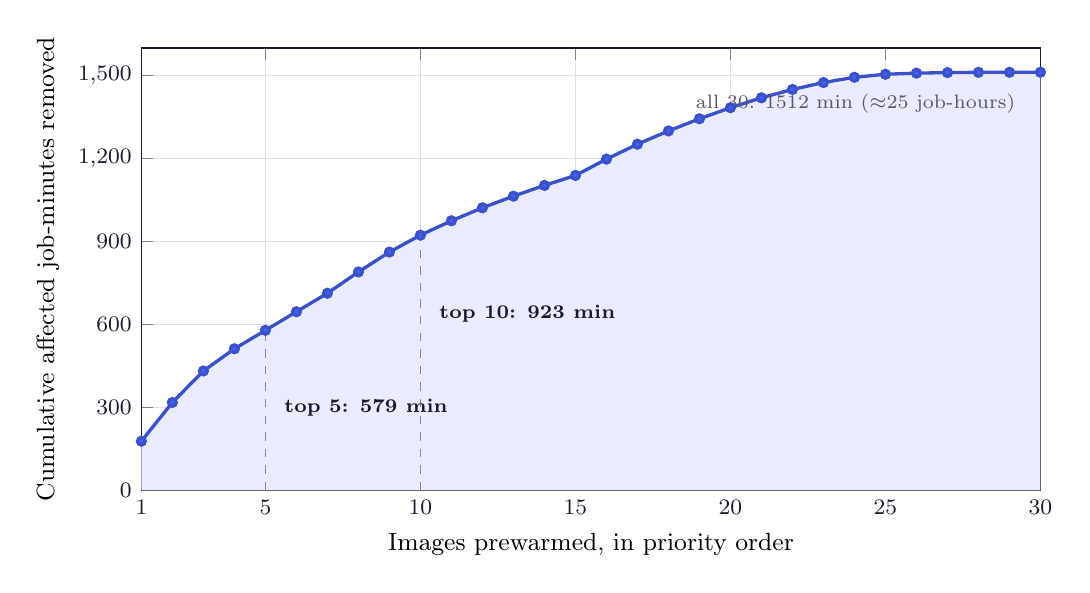
\begin{tikzpicture}[font=\sffamily]
\begin{axis}[
  width=13cm, height=7.2cm,
  xlabel={Images prewarmed, in priority order},
  ylabel={Cumulative affected job-minutes removed},
  xmin=1, xmax=30, ymin=0, ymax=1600,
  xtick={1,5,10,15,20,25,30},
  ytick={0,300,600,900,1200,1500},
  axis line style={INK},
  every axis label={INK},
  tick label style={INK, font=\footnotesize},
  label style={font=\small},
  grid=major, grid style={SUB!18},
  clip=false,
]
\addplot[name path=curve, draw=none] coordinates {
  (1,178) (2,318) (3,432) (4,512) (5,578.81)
  (6,646) (7,713) (8,790) (9,862) (10,923.02)
  (11,975) (12,1022) (13,1064) (14,1103) (15,1139)
  (16,1198) (17,1252) (18,1300) (19,1344) (20,1384)
  (21,1420) (22,1450) (23,1475) (24,1494) (25,1505)
  (26,1509) (27,1511) (28,1512) (29,1512.2) (30,1512.28)
};
\path[name path=base] (axis cs:1,0) -- (axis cs:30,0);
\addplot[COLD!12] fill between[of=curve and base];
\addplot[very thick, COLD!85!black, mark=*, mark options={fill=COLD, scale=0.7}] coordinates {
  (1,178) (2,318) (3,432) (4,512) (5,578.81)
  (6,646) (7,713) (8,790) (9,862) (10,923.02)
  (11,975) (12,1022) (13,1064) (14,1103) (15,1139)
  (16,1198) (17,1252) (18,1300) (19,1344) (20,1384)
  (21,1420) (22,1450) (23,1475) (24,1494) (25,1505)
  (26,1509) (27,1511) (28,1512) (29,1512.2) (30,1512.28)
};
\draw[dashed, SUB!70] (axis cs:5,0) -- (axis cs:5,578.81);
\draw[dashed, SUB!70] (axis cs:10,0) -- (axis cs:10,923.02);
\node[anchor=west, font=\scriptsize\bfseries, text=INK] at (axis cs:5.3,300)
  {top 5: 579 min};
\node[anchor=west, font=\scriptsize\bfseries, text=INK] at (axis cs:10.3,640)
  {top 10: 923 min};
\node[anchor=east, font=\scriptsize, text=SUB] at (axis cs:29.5,1400)
  {all 30: 1512 min (\(\approx\)25 job-hours)};
\end{axis}
\end{tikzpicture}
\end{document}
